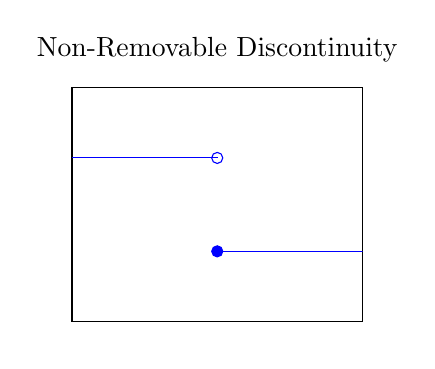
\begin{tikzpicture}
	\begin{axis}[
			axis lines        = box,
			xmin              = -5,
			xmax              = 5,
			ymin              = -5,
			ymax              = 5,
			xtick             = \empty,
			ytick             = \empty,
			xlabel            = \empty,
			ylabel            = \empty,
			trig format plots = rad,
			width             = 15em,
			title             = {Non-Removable Discontinuity}
		]

		\addplot [
			smooth,
			color=blue,
			domain=-5:0
		]{2};

		\addplot [
			smooth,
			color=blue,
			domain=0:5
		]{-2};

		\addplot [
			color=blue,
			mark=o
		]coordinates {(0,2)};

		\addplot [
			color=blue,
			mark=*
		]coordinates {(0,-2)};

	\end{axis}
\end{tikzpicture}

